
\begin{frame}\frametitle{Modelling of hadron collisions}
\small\centering

want to do physics at hadron colliders?

need a good understanding of incoming hadrons

\myskip
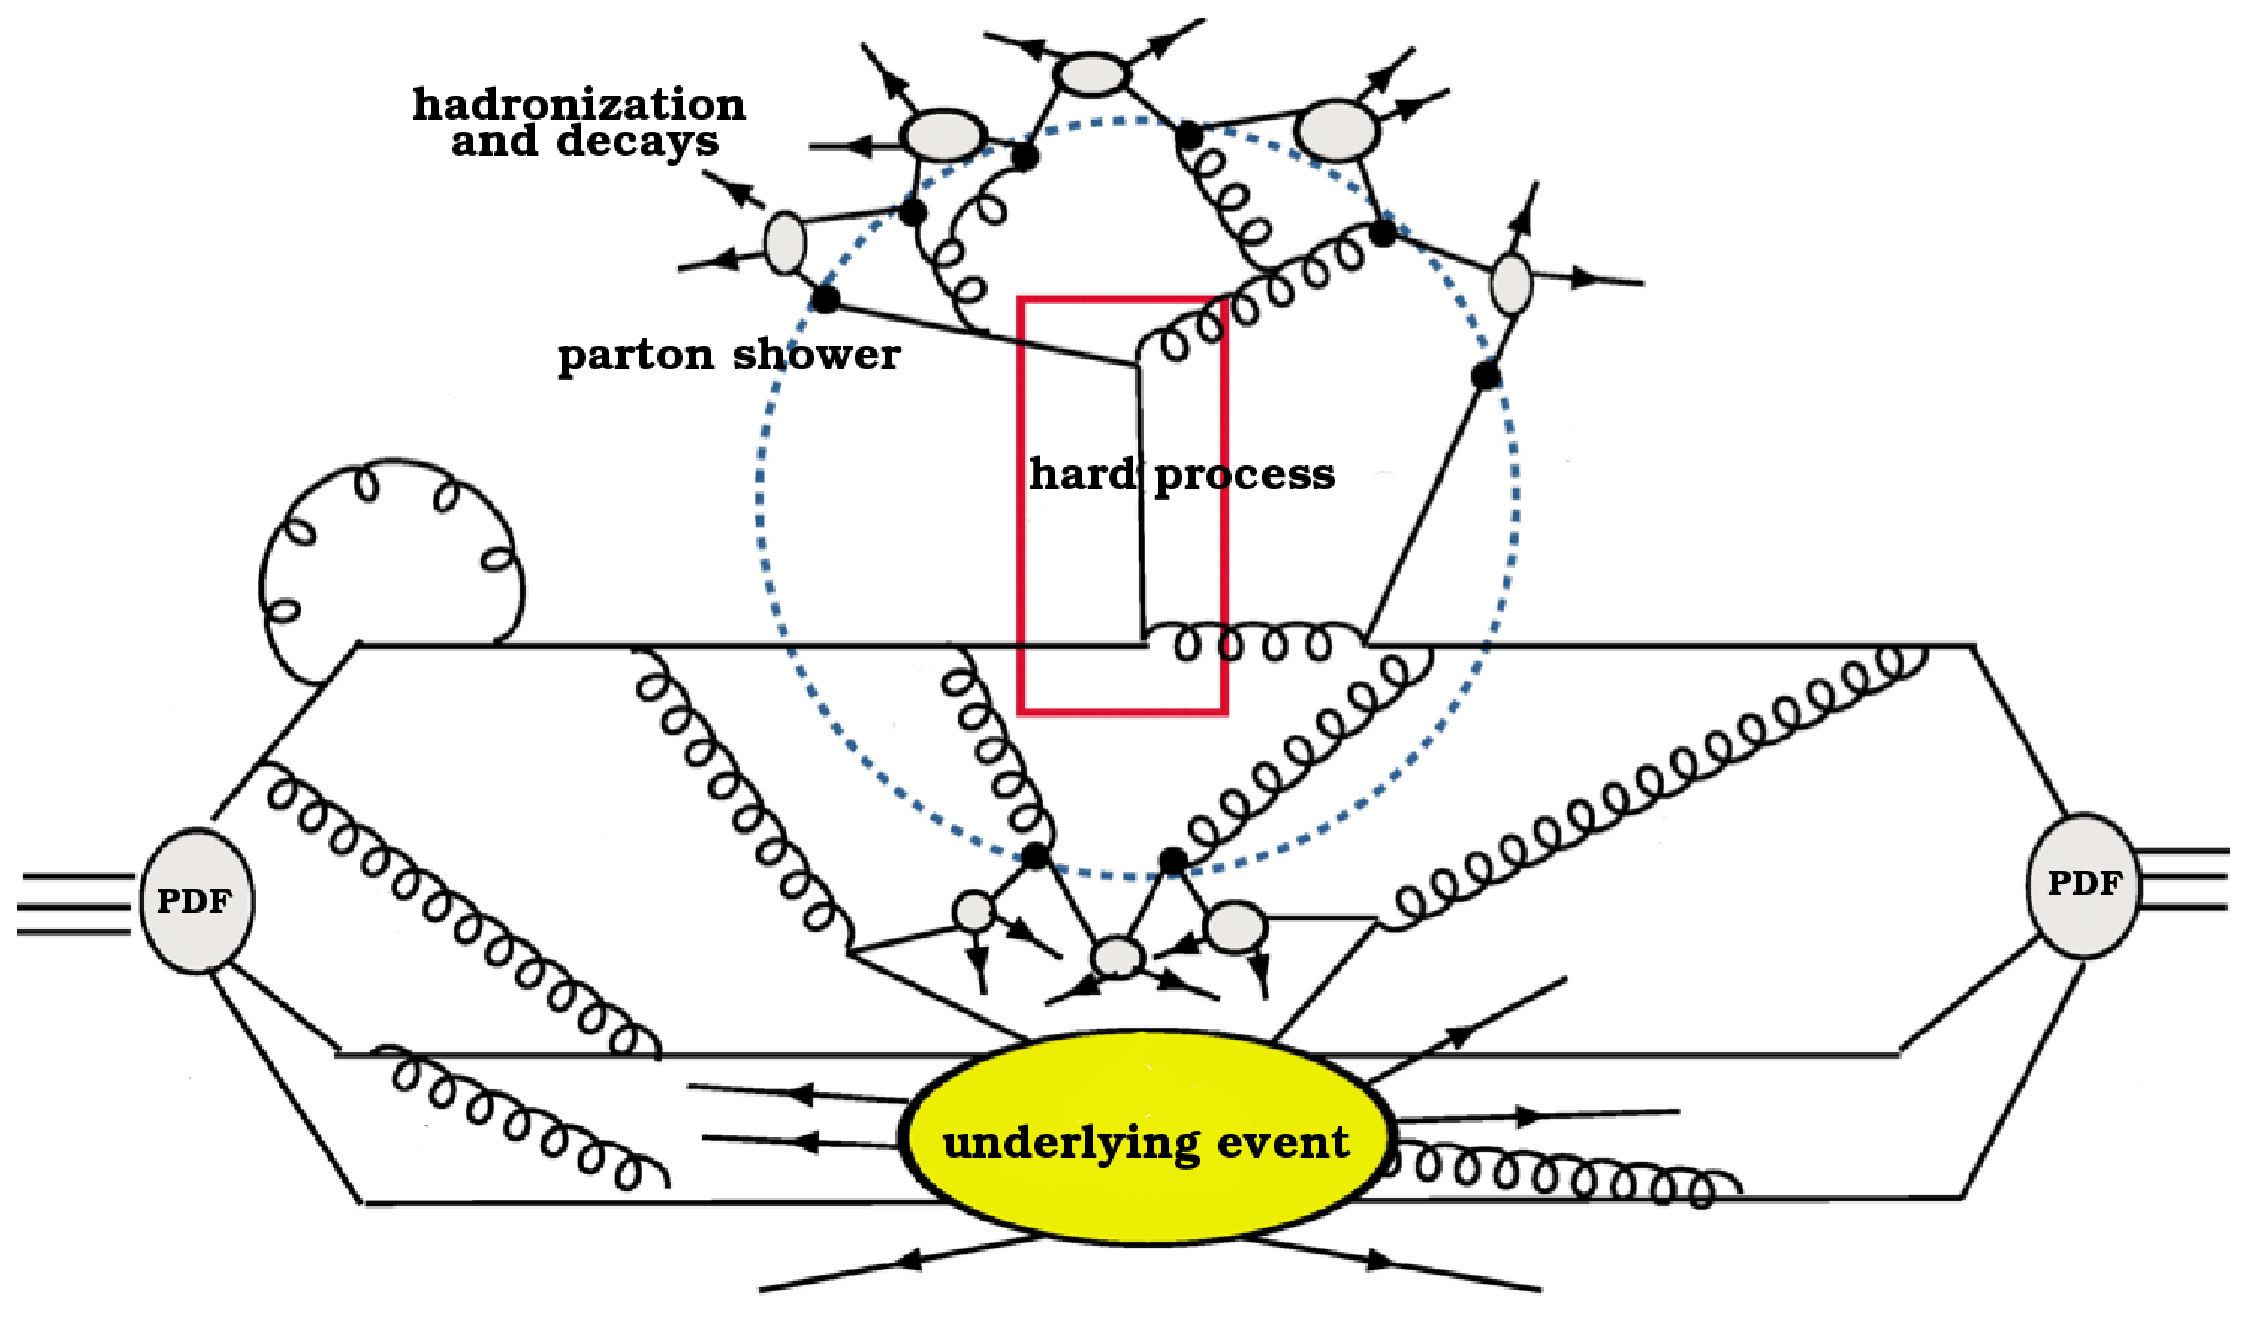
\includegraphics[width=.7\textwidth]{../montecarlo/figures/my_collision}

\end{frame}

%%%% EVENT1
\FullBackgroundPicture{../montecarlo/figures/event1}
\begin{frame}\frametitle{Modelling of hadron collisions}

\begin{flushright}\tiny Drawings from~\cite{Gieseke}\end{flushright}

\centering\myskip
%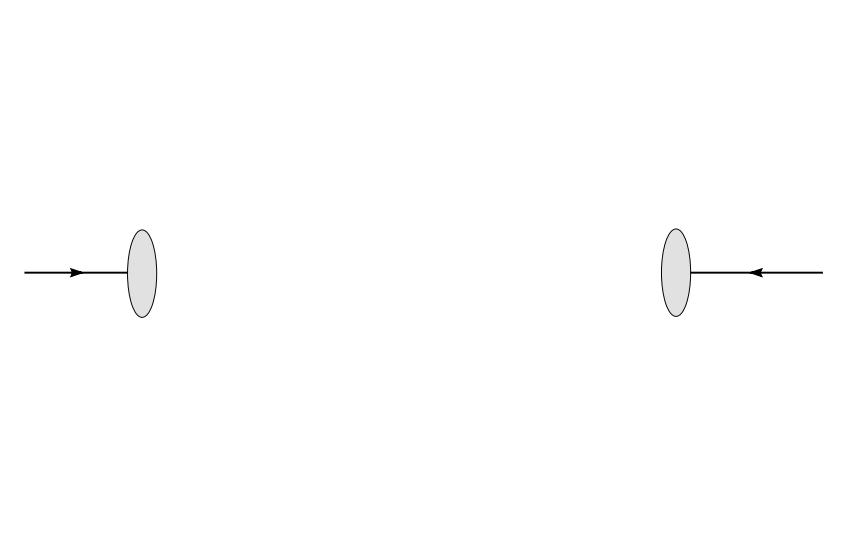
\includegraphics[height=0.8\textheight]{../montecarlo/figures/event1}

$E(p_1)=4\tev$ \hspace{.3\paperwidth} $E(p_2)=4\tev$

\vspace{.3\paperheight}

Quarks are distributed according to PDFs inside the proton\\
{\LARGE $\Downarrow$}\\
intial energy unknown

\end{frame}


%%%% EVENT1
\FullBackgroundPicture{../montecarlo/figures/event2}
\begin{frame}\frametitle{Hard scattering of two partons}
%\begin{flushright}\tiny Drawings from~\cite{Gieseke}\end{flushright}
\centering\myskip
%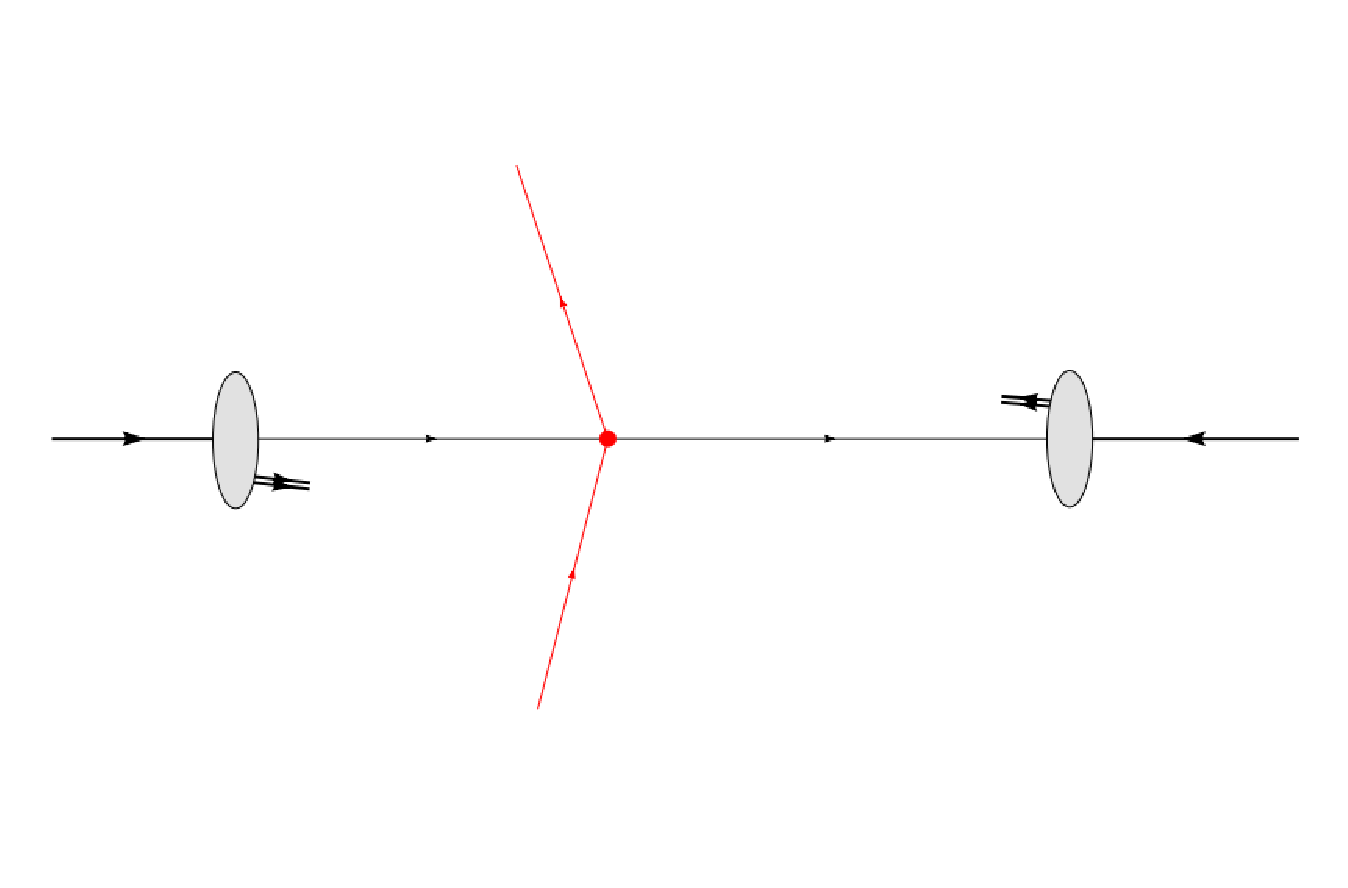
\includegraphics[height=0.8\textheight]{../montecarlo/figures/event2}


\vspace{.4\paperheight}

{\cccolor asymptotic freedom}: high energy $\longleftrightarrow$ low \alphas\\
{\LARGE $\Downarrow$}\\
(fixed order) pQCD

\end{frame}

%%%% EVENT1
\FullBackgroundPicture{../montecarlo/figures/event3}
\begin{frame}\frametitle{Parton showering}
%\begin{flushright}\tiny Drawings from~\cite{Gieseke}\end{flushright}
\centering\myskip
%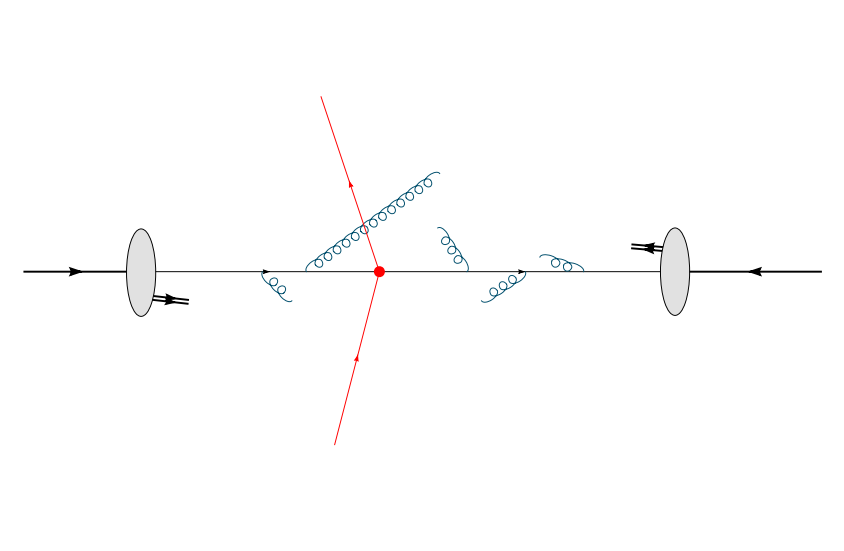
\includegraphics[height=0.8\textheight]{../montecarlo/figures/event3}

\vspace{.4\paperheight}

%real radiative corrections to any inclusive quantity

QCD emission: $q\to gq$, $g\to gg$, $g\to q\bar{q}$\\
{\LARGE $\Downarrow$}\\
higher-order corrections 

\end{frame}

%%%% EVENT1
\FullBackgroundPicture{../montecarlo/figures/event4}
\begin{frame}\frametitle{Parton showering}
\centering\myskip
%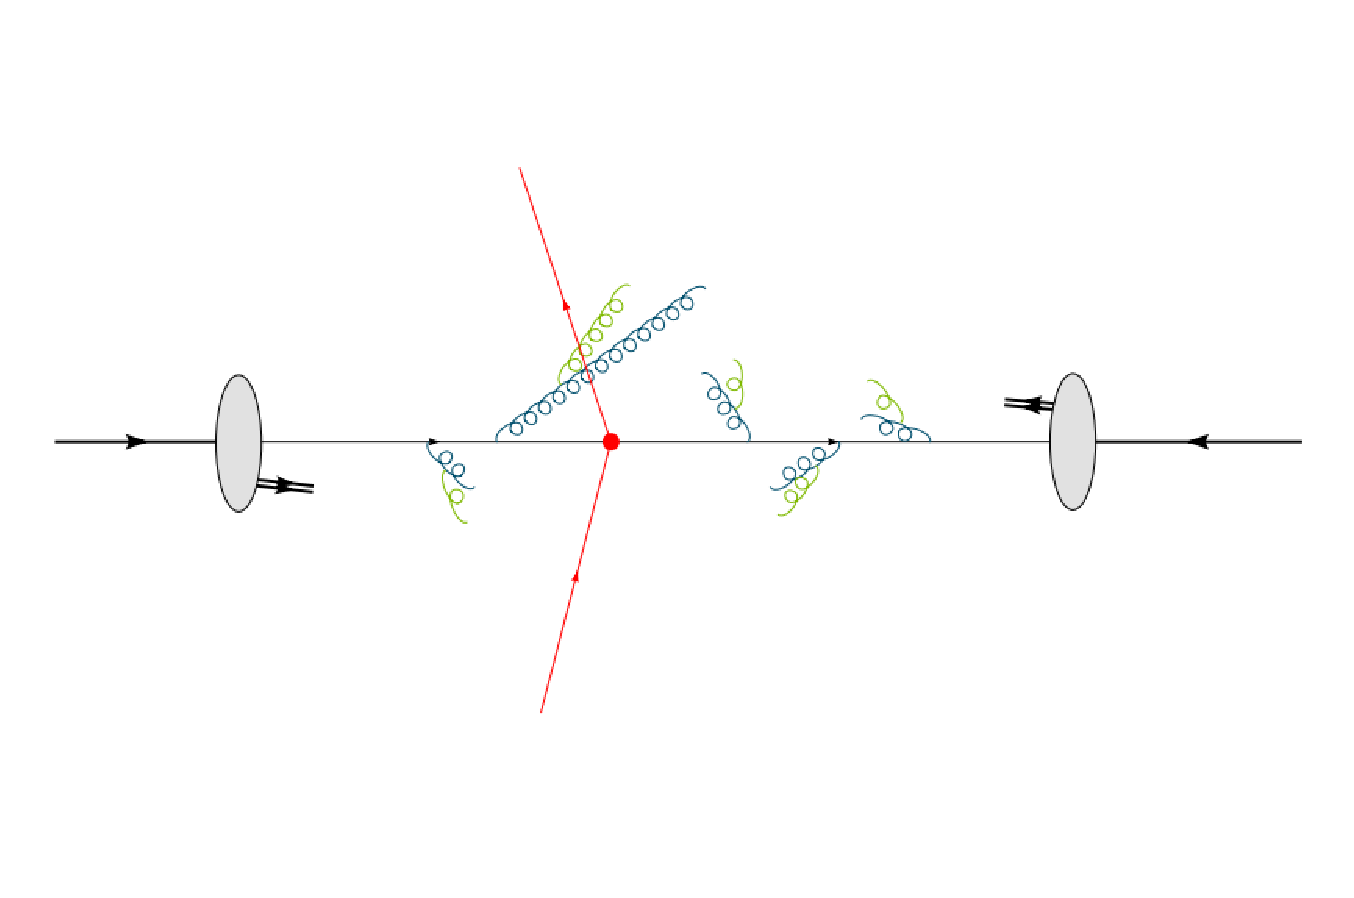
\includegraphics[height=0.8\textheight]{../montecarlo/figures/event4}

\vspace{.4\paperheight}

%real radiative corrections to any inclusive quantity

QCD emission: $q\to gq$, $g\to gg$, $g\to q\bar{q}$\\
{\LARGE $\Downarrow$}\\
higher-order corrections 

%\begin{flushright}\tiny Drawings from~\cite{Gieseke}\end{flushright}

\end{frame}

%%%% EVENT1
\FullBackgroundPicture{../montecarlo/figures/event5}
\begin{frame}\frametitle{Hadronization}
\centering\myskip
%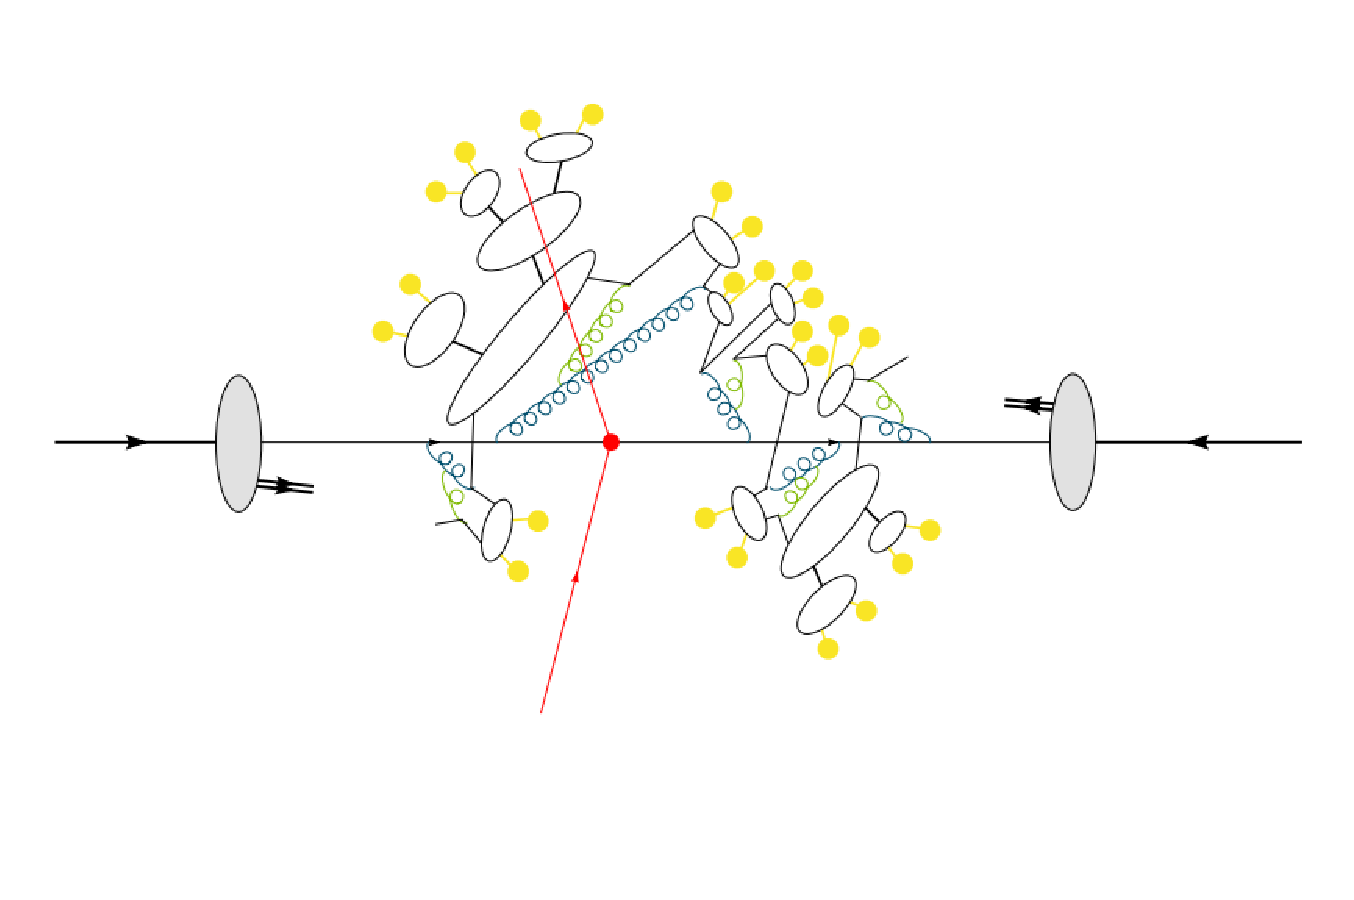
\includegraphics[height=0.8\textheight]{../montecarlo/figures/event5}


\vspace{.4\paperheight}

%\begin{flushright}\tiny Drawings from~\cite{Gieseke}\end{flushright}

\end{frame}

%%%% EVENT1
\FullBackgroundPicture{../montecarlo/figures/event6}
\begin{frame}\frametitle{Final particle decays}
\centering\myskip
%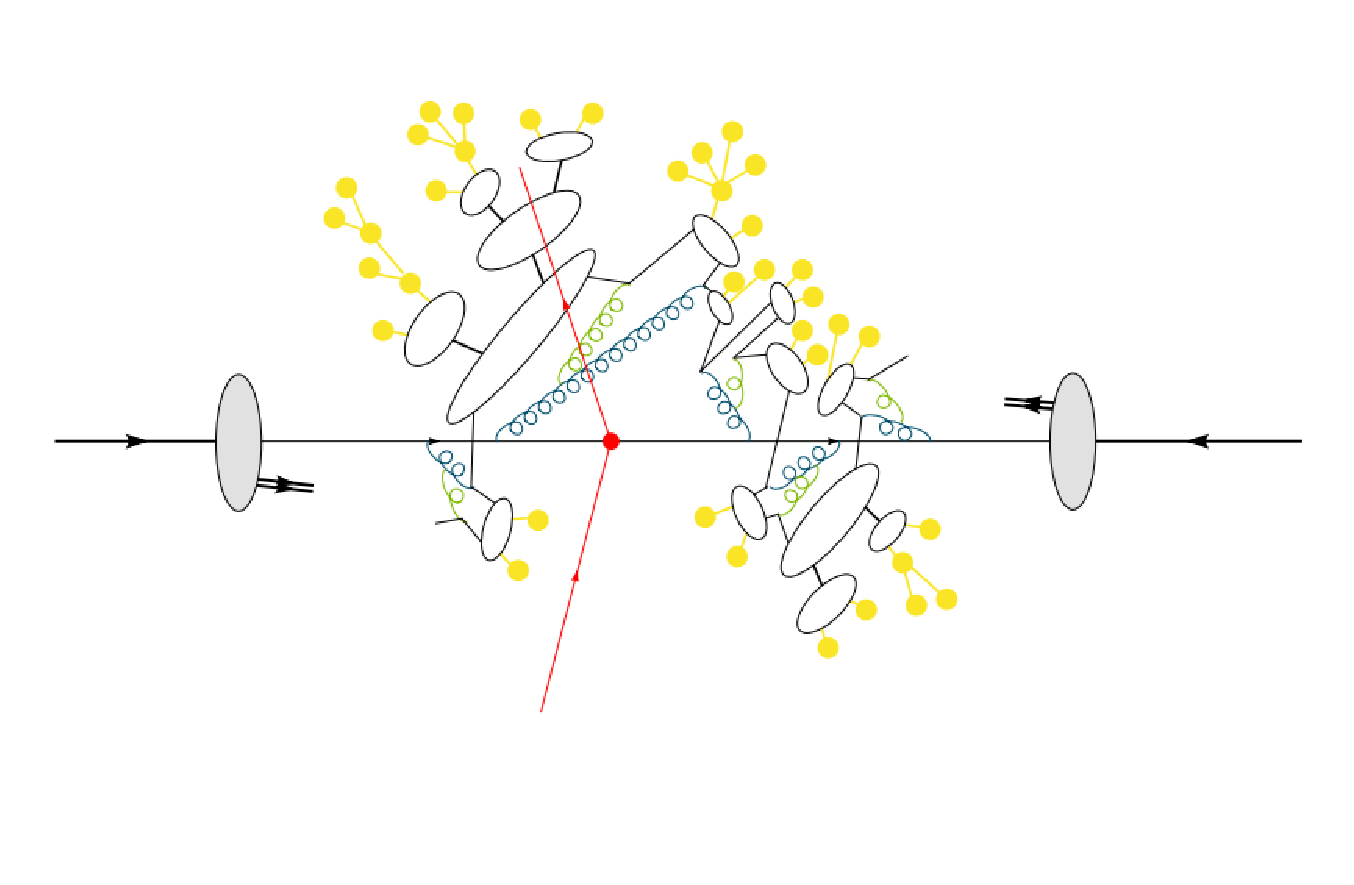
\includegraphics[height=0.8\textheight]{../montecarlo/figures/event6}


\vspace{.4\paperheight}

%\begin{flushright}\tiny Drawings from~\cite{Gieseke}\end{flushright}

\end{frame}

%%%% EVENT1
\FullBackgroundPicture{../montecarlo/figures/event7}
\begin{frame}\frametitle{Underlying event simulation}
\centering\myskip
%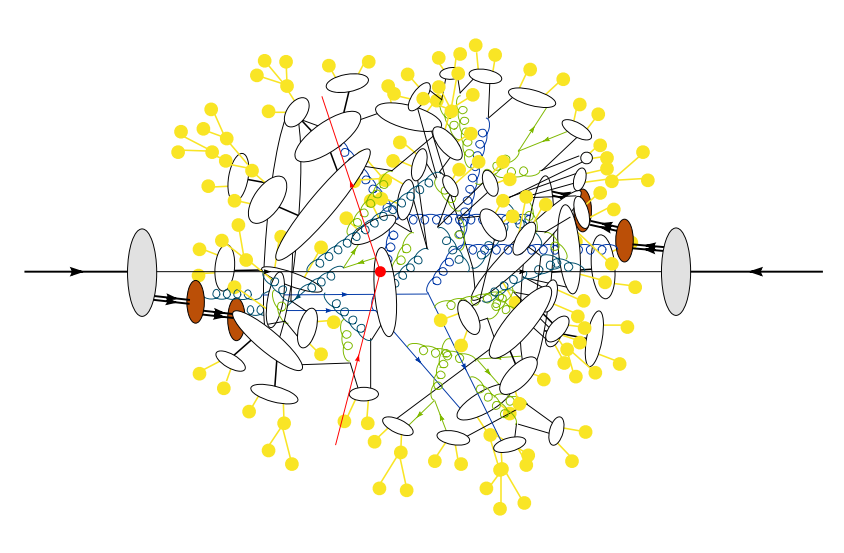
\includegraphics[height=0.8\textheight]{../montecarlo/figures/event7}


\vspace{.4\paperheight}

%\begin{flushright}\tiny Drawings from~\cite{Gieseke}\end{flushright}

\end{frame}

